% ABOUTME: Deep learning dataset justification and single-factor ablation studies.
% ABOUTME: Covers window length, padding trade-offs, RUL clipping, regularisation, inputs, and hybrid branches.
\section{Dataset Choices and Ablation Studies}
\label{sec:ablations}

This section first justifies how the sequence data are built, then removes
or changes one design choice of the selected Transformer at a time and
measures, by cross validation on the training engines only, what each choice
was worth. All numbers are from \texttt{results/ablations.csv} and
\texttt{results/ablation\_window\_unpadded.csv}, produced by
\texttt{scripts/run\_ablations.py} and \texttt{notebooks/08\_ablations.ipynb}.

\subsection{DL Dataset Choices}
\label{sec:dl-data-choices}

\textbf{Window length, coverage and padding.}
Training engines run to failure and are long (128 to 362 cycles), while test
engines are cut off before failure; the shortest test engine has 31 cycles.
The first $w-1$ cycles of every engine have less than $w$ cycles of history,
and we left pad them with copies of the engine's first reading
(Section~\ref{sec:dl-setup}). The window length therefore trades history
against padding:
\begin{itemize}
  \item At $w = 15$, 1,400 training windows (6.8\% of cycles) are padded, and
  every test engine is scored on real history.
  \item At $w = 30$, 2,900 training windows (14.1\%) are padded, and every
  test engine is still scored on real history, because 30 cycles fit within
  the shortest test engine.
  \item At $w = 50$, 4,900 training windows (23.8\%) are padded, and seven test
  engines (units 1, 2, 14, 22, 25, 39 and 85) have fewer than 50 cycles, so
  their scored window is padded too.
\end{itemize}
Fig.~\ref{fig:ablation-coverage}(a) shows this trade-off.

\begin{figure*}[t]
  \centering
  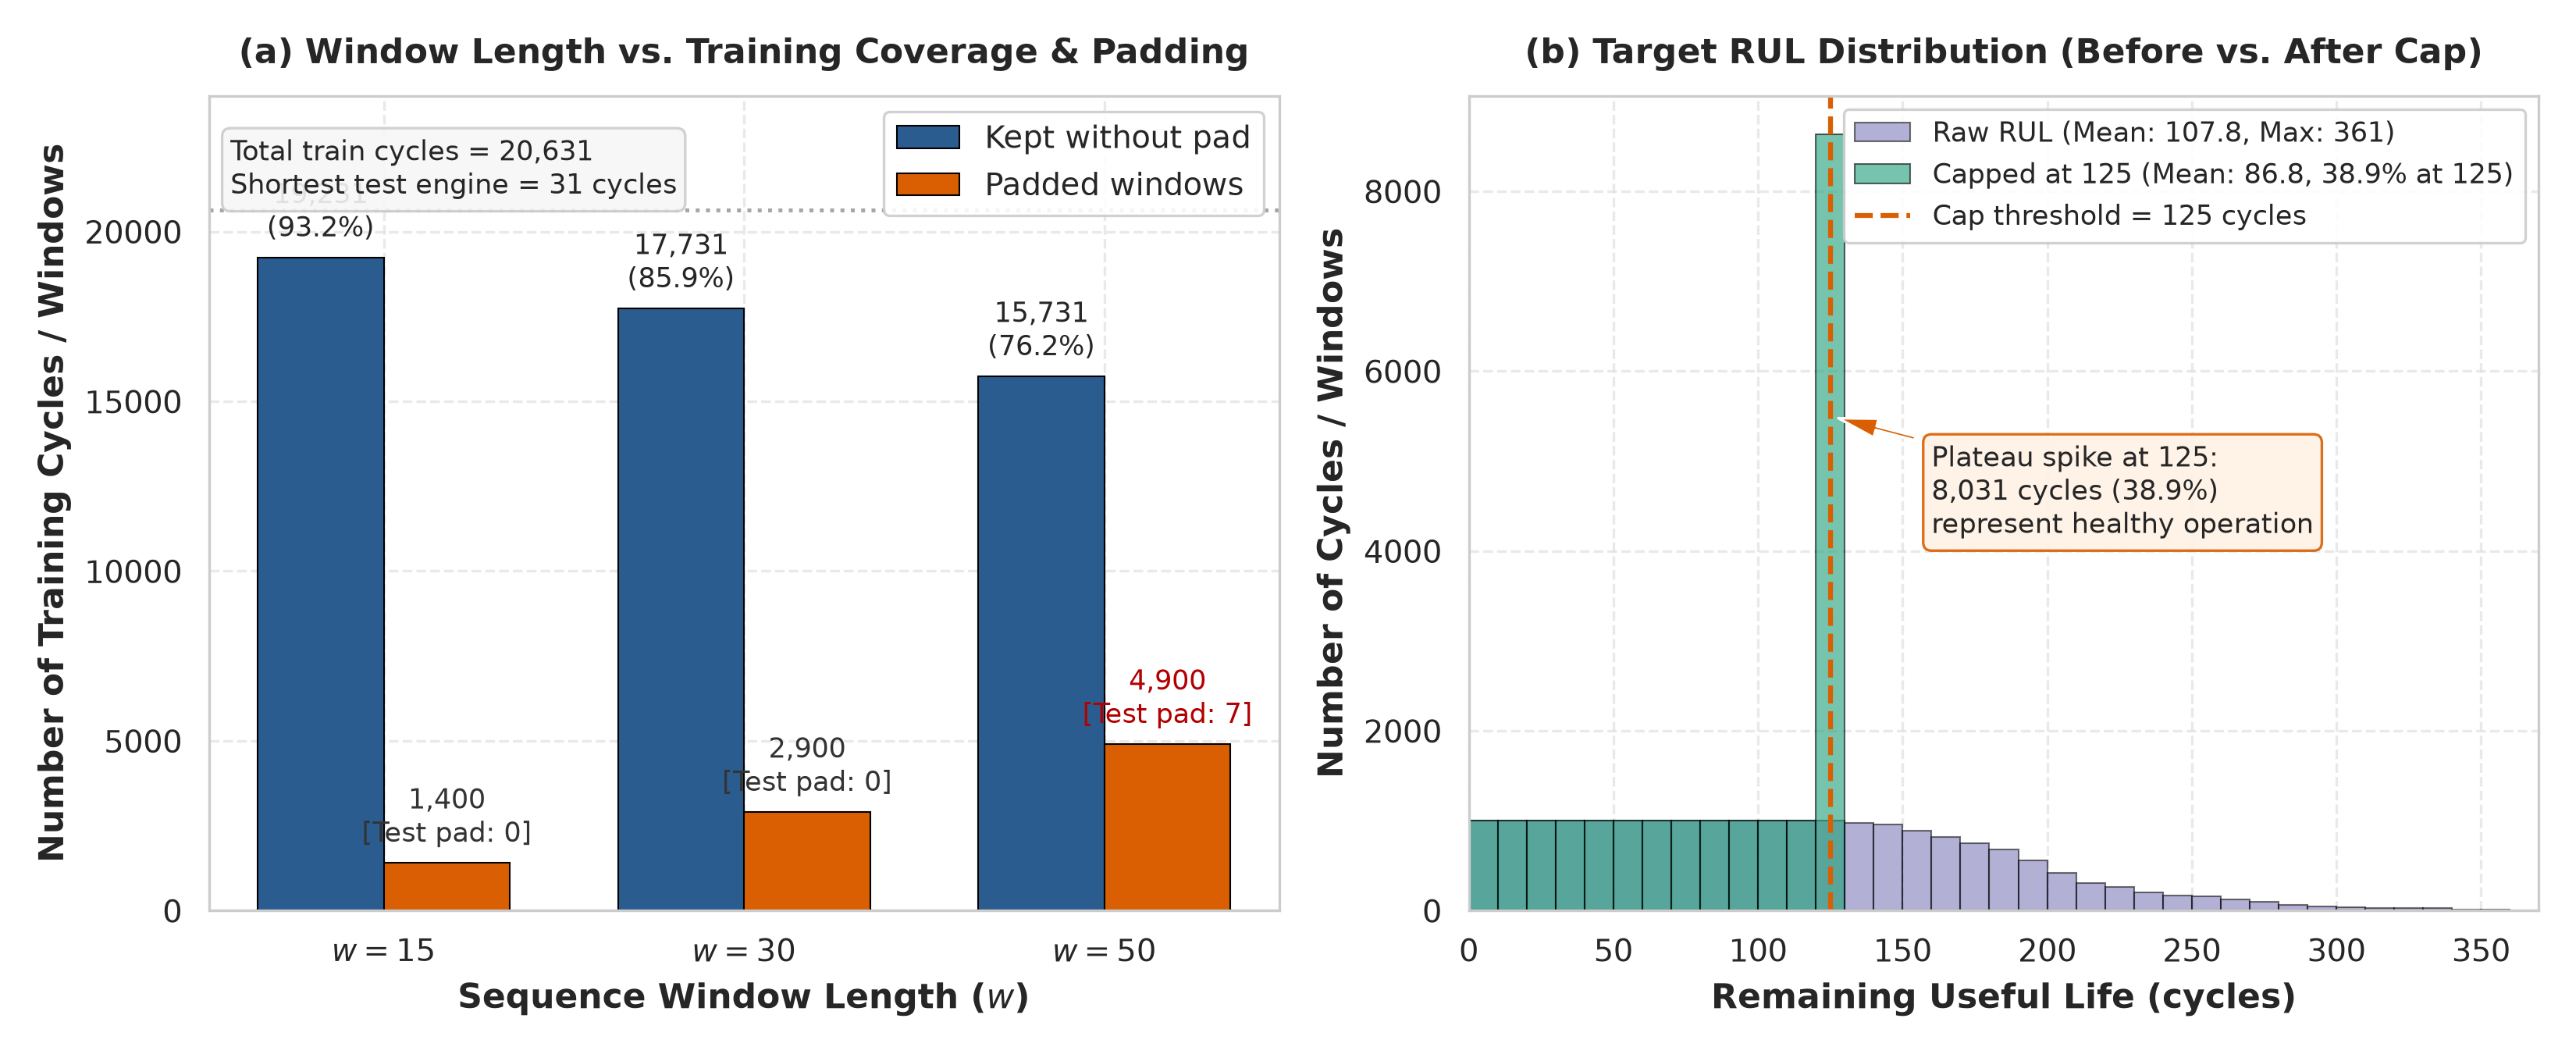
\includegraphics[width=\textwidth]{../figures/ablation_coverage_padding.png}
  \caption{(a) Training windows padded and test engines with less history
  than the window, for each window length. (b) Training RUL before and after
  clipping at 125 cycles; 38.9\% of training cycles fall on the plateau.}
  \label{fig:ablation-coverage}
\end{figure*}

\textbf{Target cap at 125 cycles.}
Uncapped training RUL runs from 0 to 361 cycles (mean $107.81 \pm 68.88$).
Early in life the sensors do not yet show wear, so engines with very
different remaining lives look alike. Capping at 125 clips 8,031 training
cycles (38.9\%) onto a plateau and reduces the standard deviation of the
target to 41.67 cycles (Fig.~\ref{fig:ablation-coverage}(b)).

\textbf{Operating regime.}
FD001 has a single operating condition: settings 1 and 2 have standard
deviations of 0.0022 and 0.00029 and setting 3 is always 100. Standardising
sensors per regime and standardising them globally on the training engines
therefore coincide.

\subsection{Ablation Method}
\label{sec:ablation-methodology}

Each ablation changes exactly one factor of the selected Transformer
($w = 30$, cap 125, dropout 0.1, weight decay $10^{-4}$, early stopping with
patience 10 on 20\% of each fold's training engines, learning rate
$10^{-3}$, 14 sensors) and is scored with the same five engine folds,
against RUL capped at 125 on every cycle. Removing early stopping means
training for 40 epochs and keeping the last epoch's weights; the training
loop otherwise restores the best early stopping epoch.

Two sources of noise limit what a difference can show. The first is the
fold spread. The second is the run itself: the same baseline configuration
gives a CV RMSE of 13.00 with default PyTorch threads, $13.17 \pm 0.72$ with
one thread, and 13.28 in Table~\ref{tab:dl-cv}, because the order of
floating point operations changes the training trajectory. The rows were
produced in two runs, so each row is compared only with the baseline of its
own run (Table~\ref{tab:ablations}). We treat a difference as evidence only
when it is larger than the fold standard deviation of both rows and than
this run to run variation of about 0.3 cycles.

\begin{table*}[t]
\centering
\caption{Single-factor ablations: five fold engine cross validation, RUL
capped at 125, mean $\pm$ standard deviation over folds. $\Delta$ is the RMSE
minus that of the baseline in the same run. Late RMSE covers cycles with
true RUL $\le 50$. The last row is scored against the true, uncapped RUL and
is not comparable with the others.}
\label{tab:ablations}
\footnotesize
\begin{tabular}{llrrrrr}
\hline
Ablation & Changed factor & RMSE & $\Delta$ & MAE & Late RMSE & Score $S$ \\
\hline
\multicolumn{7}{l}{\emph{Run 1: default threads}} \\
Baseline (Transformer) & -- & 13.00 $\pm$ 0.67 & -- & 9.30 & 7.85 & 12,657 \\
Window & $w = 15$ & 16.96 $\pm$ 0.48 & $+3.96$ & 12.36 & 14.18 & 39,447 \\
Window & $w = 50$ & 11.34 $\pm$ 0.52 & $-1.66$ & 8.06 & 6.42 & 9,153 \\
Regularisation & no dropout & 13.54 $\pm$ 0.84 & $+0.54$ & 9.73 & 8.14 & 14,145 \\
Regularisation & no weight decay & 13.47 $\pm$ 0.71 & $+0.46$ & 9.52 & 7.69 & 14,552 \\
Inputs & top 3 SHAP sensors & 18.70 $\pm$ 1.50 & $+5.70$ & 13.25 & 15.48 & 642,025 \\
Inputs & top 5 SHAP sensors & 15.44 $\pm$ 1.12 & $+2.44$ & 10.66 & 11.64 & 36,796 \\
Hybrid & sequence branch only & 13.34 $\pm$ 0.34 & $+0.33$ & 9.43 & 7.34 & 14,198 \\
Hybrid & feature branch only & 15.29 $\pm$ 0.91 & $+2.29$ & 11.32 & 12.33 & 34,550 \\
Hybrid & both branches & 13.47 $\pm$ 0.53 & $+0.47$ & 9.77 & 7.53 & 14,500 \\
\hline
\multicolumn{7}{l}{\emph{Run 2: one thread}} \\
Baseline (Transformer) & -- & 13.17 $\pm$ 0.72 & -- & 9.40 & 8.36 & 14,336 \\
Regularisation & no early stopping & 15.65 $\pm$ 0.66 & $+2.48$ & 10.98 & 9.74 & 27,410 \\
Regularisation & all three off & 16.00 $\pm$ 1.13 & $+2.83$ & 11.48 & 10.11 & 25,032 \\
Target & no cap, predictions clipped & 15.42 $\pm$ 1.61 & $+2.25$ & 9.40 & 10.79 & 33,654 \\
Target & no cap, true RUL & 38.57 $\pm$ 2.25 & n/c & 26.92 & 11.00 & -- \\
\hline
\end{tabular}
\end{table*}

\subsection{Findings}
\label{sec:ablation-discussion}

Fig.~\ref{fig:ablation-comparison} shows each row's difference from its own
baseline.

\begin{figure}[t]
  \centering
  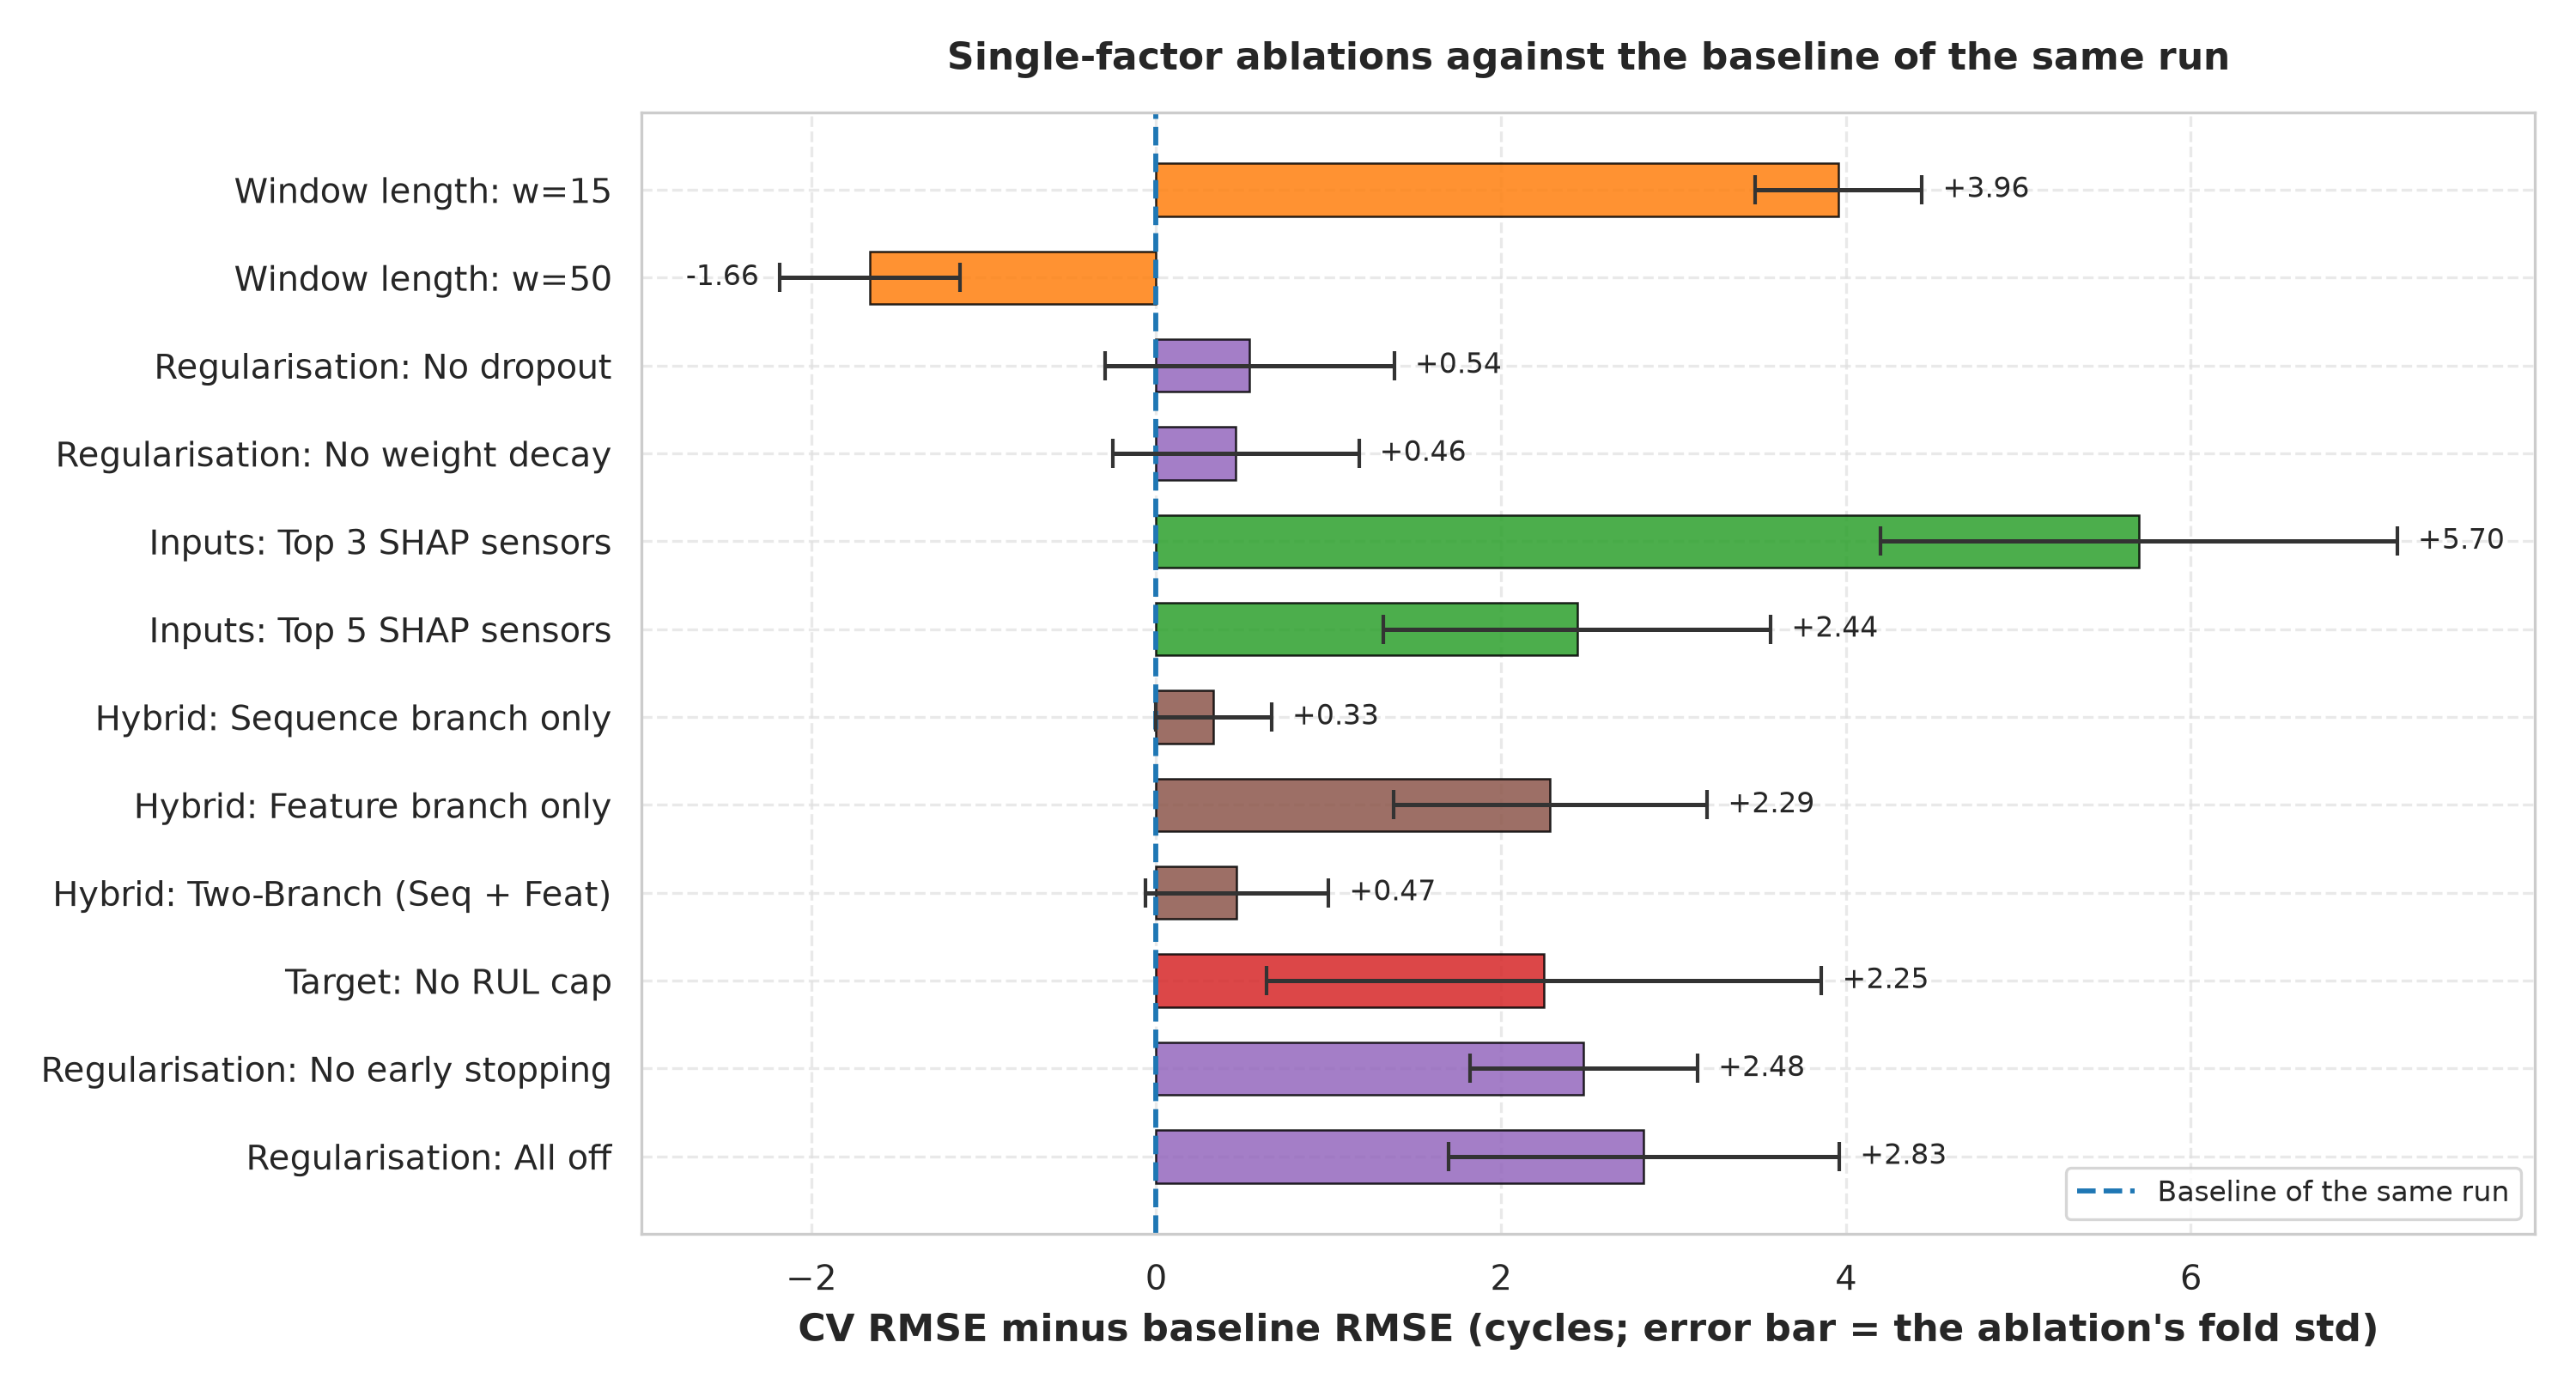
\includegraphics[width=\columnwidth]{../figures/ablation_cv_comparison.png}
  \caption{CV RMSE of each ablation minus the baseline of the same run. Error
  bars are the ablation's fold standard deviation.}
  \label{fig:ablation-comparison}
\end{figure}

\textbf{Window length.} Fifteen cycles is clearly too short: RMSE rises by
3.96 cycles and late RMSE from 7.85 to 14.18. Fifty cycles is clearly
better: RMSE falls by 1.66 cycles, 2.5 to 3 fold standard deviations,
and late RMSE to 6.42. Because a padded window reveals how early in life an
engine is, we checked whether padding explains the gain by scoring only
cycles $\ge 50$, where no window of either length is padded. There, in one
run, $w = 50$ still reaches $11.96 \pm 0.59$ against $14.19 \pm 0.77$ for
$w = 30$, and is better on every fold. A longer history genuinely helps on
cross validation. We did not switch to $w = 50$: the window was fixed before
the test set was opened (Section~\ref{sec:dl-results}), and these ablations
were run afterwards, so changing it now would be a choice made after seeing
test results. It is the clearest improvement this study found and a
limitation of the selected model.

\textbf{Target cap.} Training without the cap is worse even when its
predictions are clipped at 125 and scored like every other row: RMSE rises
by 2.25 cycles and the fold spread doubles. Scored against its own target,
the true uncapped RUL, its RMSE is 38.57, because early cycles of healthy
engines carry RUL of up to 361 cycles that the sensors do not show.

\textbf{Regularisation.} Removing dropout or weight decay alone changes RMSE
by $+0.54$ and $+0.46$ cycles, less than the fold standard deviations of 0.84
and 0.71, so neither has a measurable effect. Removing early stopping is
clearly worse, by 2.48 cycles, and removing all three is worse by 2.83, about
as much as early stopping alone. Early stopping is the regulariser that
matters here.

\textbf{Inputs.} The top three SHAP sensors of Phase~1 ($s_4$, $s_{15}$,
$s_2$) are clearly not enough (RMSE $+5.70$, late RMSE 15.48). The top five
recover part of the gap but remain 2.44 cycles behind all 14 sensors.

\textbf{Hybrid branches.} The sequence branch alone with the hybrid's head
is within the fold spread of the plain Transformer ($+0.33$), and the
feature branch alone is clearly worse ($+2.29$). Adding the feature branch to
the sequence branch does not help: the two-branch hybrid is 0.14 cycles worse
overall and its late RMSE (7.53) is no better than that of the sequence
branch alone (7.34). Within this study the sensor window carries the
predictive signal and the engineered features add nothing measurable.
